\section{Hadoop Open Plataform-as-a-Service (Hops)}
In BiobankCloud, we are using our distribution of the Hadoop Filesystem (HDFS), HopsFS, to store large genomic files. HopsFS scales to store 100s of millions of files. Hops is a distribution of Apache Hadoop 2 that has a new metadata management architecture based on a shared-nothing, in-memory distributed database, see Figure \ref{fig:hop-fs_architecture}. HopsFS introduces multiple stateless NameNodes to manage the namespace metadata that is now stored in the database. HopsFS' clients and DataNodes are aware of all NameNodes in the system. HopsFS is a highly available filesystem: whenever a NameNode fails the failed operations are automatically retried by clients and the DataNodes by forwarding the failed requests to a different live NameNode. The database we use, MySQL Cluster~\cite{ronstrom2005recovery}, is similarly highly available.


\begin{figure}[!ht]
    \subfloat[HopsFS\label{subfig-1:hopsfs}]{%
      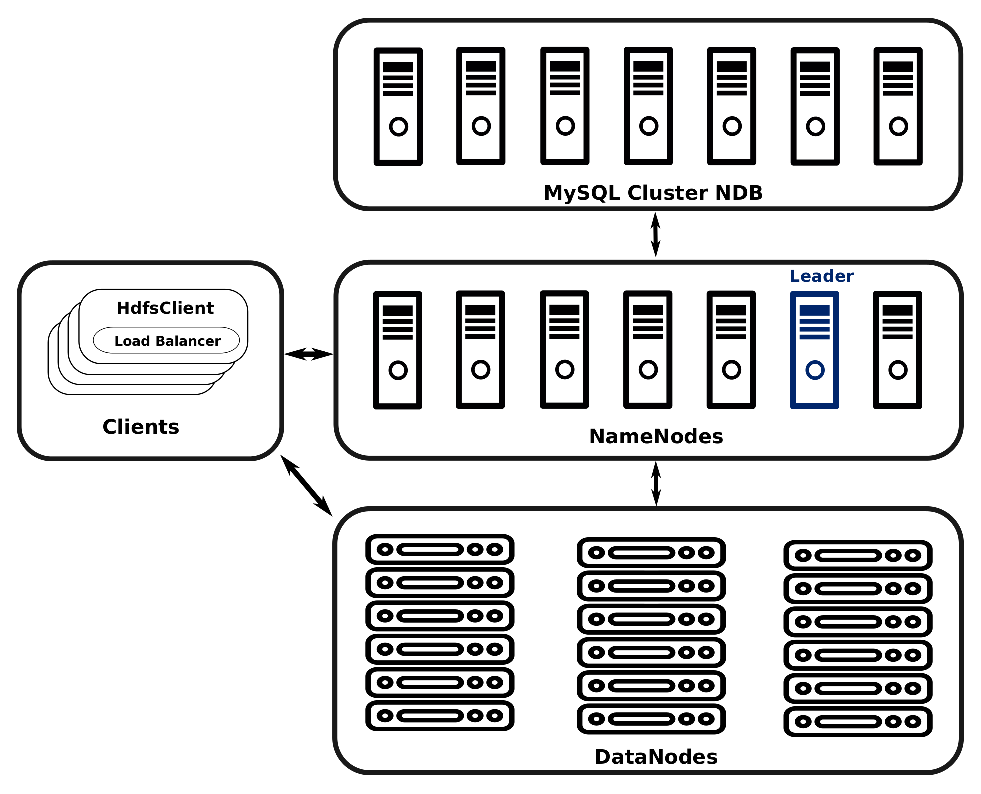
\includegraphics[width=0.48\textwidth]{./imgs/hops-fs-arch.eps}
    }
    \hfill
    \subfloat[HopsYARN\label{subfig-2:hopsyarn}]{%
      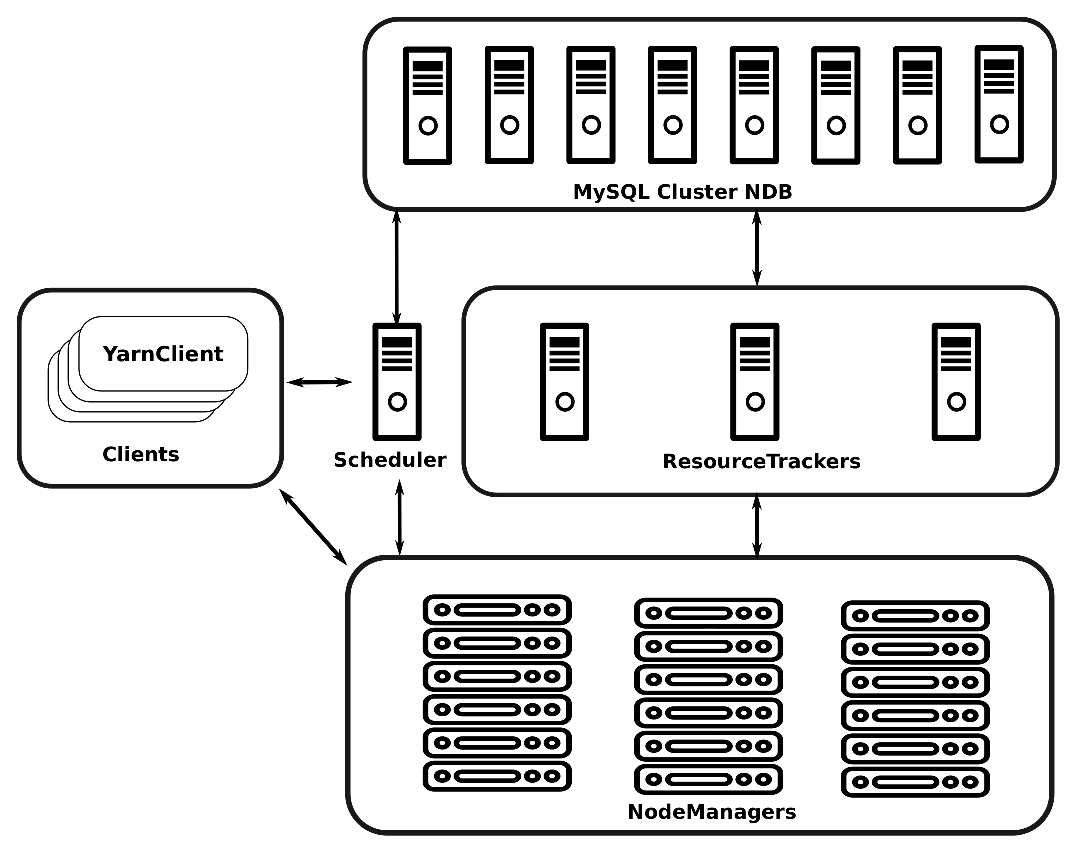
\includegraphics[width=0.48\textwidth]{./imgs/hops-yarn-arch.eps}
    }
    \caption{HopsFS and HopsYARN architectures.}
    \label{fig:dummy}
  \end{figure}
  
% \begin{figure}[th]
%  \centering
%  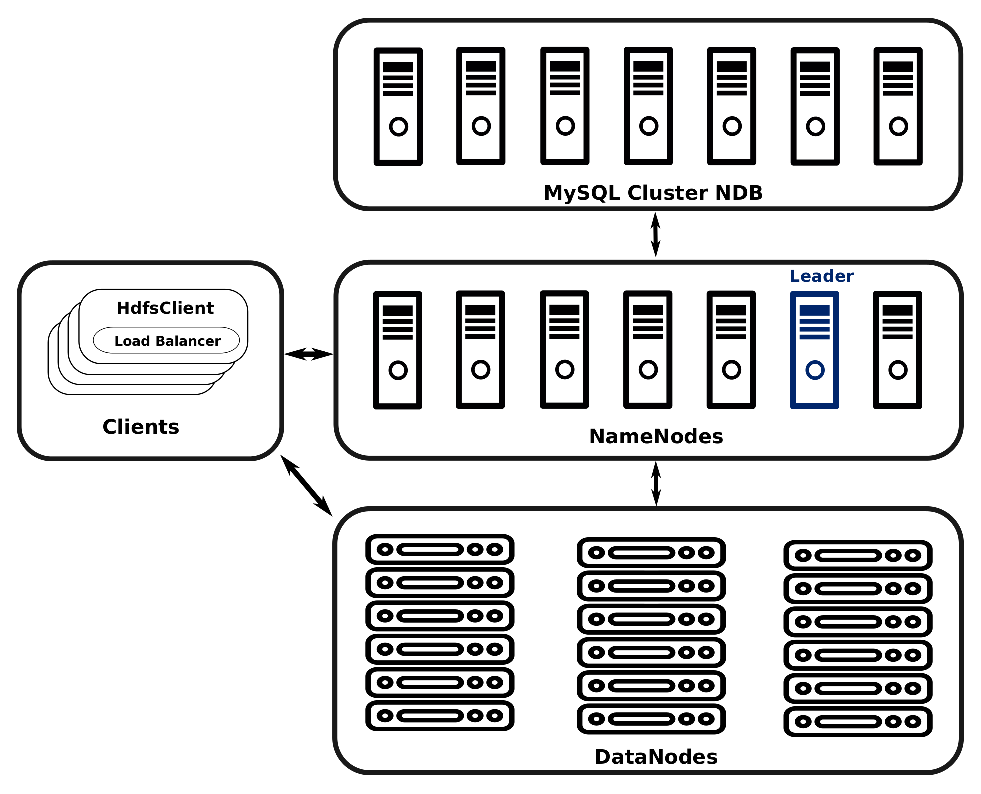
\includegraphics[width=0.9\textwidth]{./imgs/hops-fs-arch.eps}
%  % hops-fs-arch.eps: 0x0 pixel, 300dpi, 0.00x0.00 cm, bb=0 -1 455 364
% \end{figure}



We ensure the consistency of the filesystem metadata by implementing serialized transactions on well-ordered operations on metadata~\cite{hops_consistency}. We do not need Zookeeper, as we have developed a leader-election service based on the database~\cite{hopselection}. HopsFS can the amount of storage space required to store genomic data, while maintaining high availability using Reed-Solomon erasure coding, instead of the traditional three-way replication of filesystem blocks used in HDFS. Erasure-coding can reduce disk space consumption by 44\% compared to three-way replication in Apache HDFS. In HopsFS, the management of erasure coded files is implemented in the leader NameNode, triggering file repair operations when file blocks become unavailable after a failure and a balancing file blocks across DataNodes to ensure high availability.

% \begin{figure}[th]
%  \centering
%  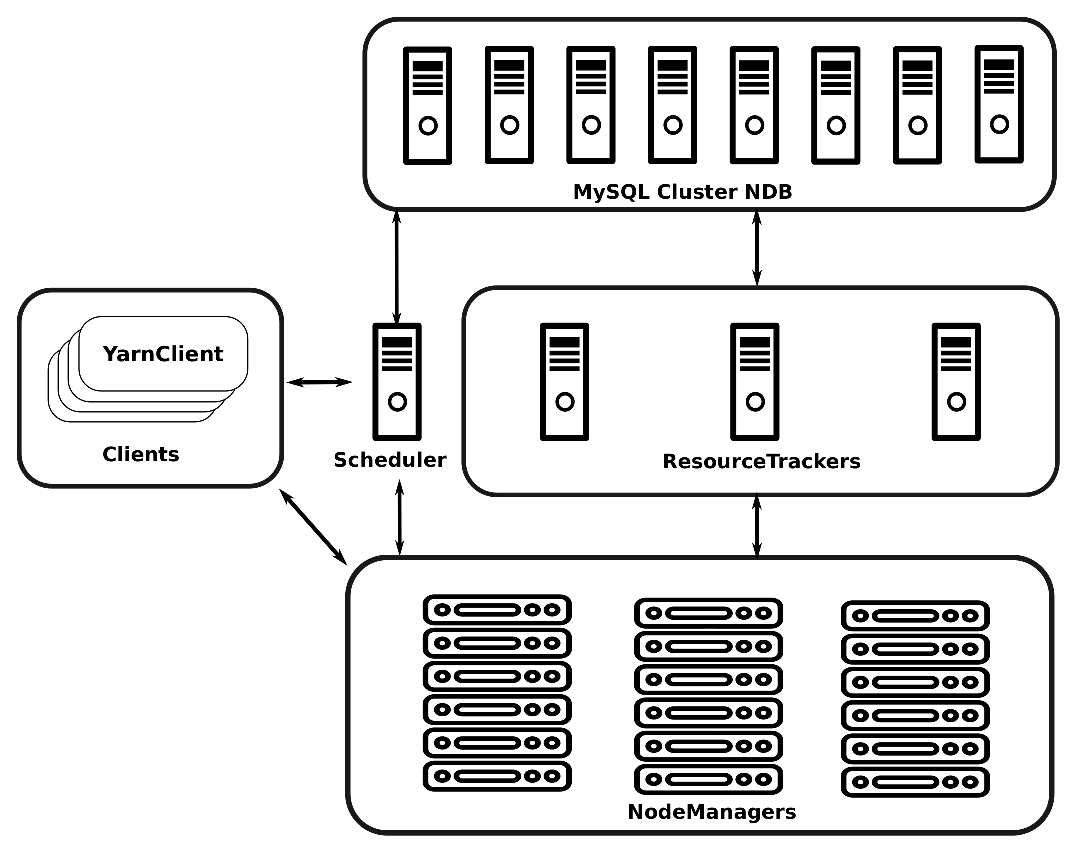
\includegraphics[width=0.9\textwidth]{./imgs/hops-yarn-arch.eps}
%  % yarn-arch.eps: 0x0 pixel, 300dpi, 0.00x0.00 cm, bb=0 0 792 612
%  \caption{HopsYARN separate scheduling from resource tracking and stores metadata in the distributed database.}
%  \label{fig:yarn-arch}
% \end{figure}

% \begin{figure}[h]
%  \centering
%  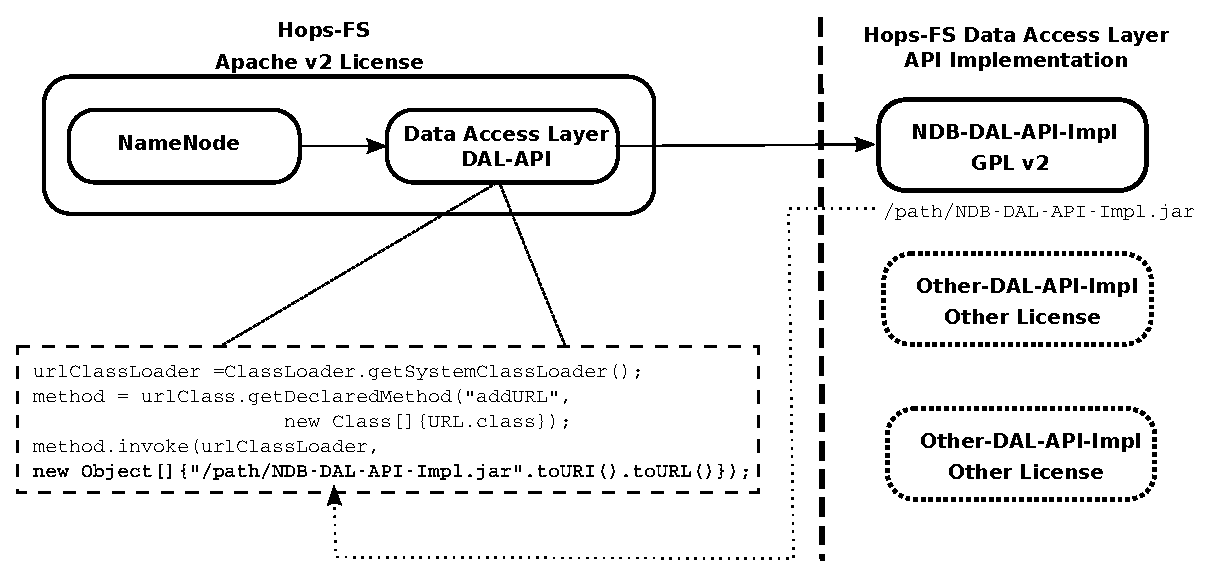
\includegraphics[width=0.9\textwidth]{./imgs/license-work-around.eps}
%  \label{fig:license-work-around}
%  \caption{Combining Apache v2 and GPL v2 Open Source Licenses}
%  % license-work-around.eps: 0x0 pixel, 300dpi, 0.00x0.00 cm, bb=0 -1 566 261
% \end{figure}


% \begin{figure}[h]
%  \centering
%  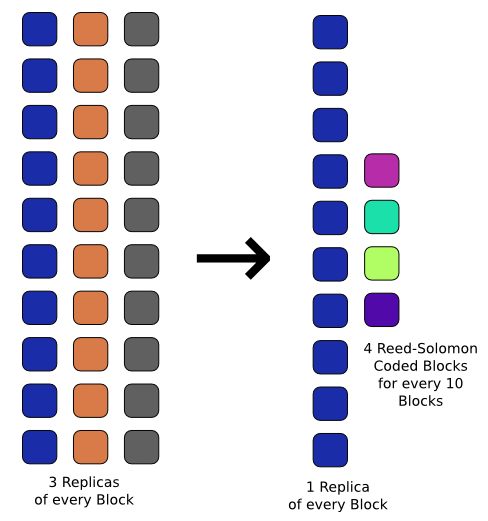
\includegraphics[width=0.5\textwidth]{./imgs/erasure-coding.png}
%  % erasure-coding.png: 0x0 pixel, 300dpi, 0.00x0.00 cm, bb=
%  \label{fig:erasure-coding}
%  \caption{Erasure coding instead of three-way replication in a HopsFS file. Here, we can reduce the number of blocks stored from 30 to 14.}
% \end{figure}

\subsubsection{Extending, Indexing and Searching Metadata}
There is a need to organize the files in such a manner that they can easily be logically grouped and searched. Typically, such functionality requires metadata for the files and directories, such as filename and last accessed time. For biological samples, much more extensive metadata is required for files that relate to biological samples. We need information such as the sample collection it belongs to, the type of sample, and donor information. BiobankCloud enables Biobankers who are not programmers to design such metadata, link it to samples, and then edit sample metadata using UI support. The metadata is transparently indexed to enable free-text searching for samples, sample collections, and studies. Our solution is based on the industry-standard Elasticsearch platform. Importantly, we guarantee the metadata's integrity by implementing an eventually consistent replication model that asynchronously copies updates to metadata from our distributed database to Elasticsearch. The distributed database uses foreign keys to guarantee the integrity of the metadata and the referrent genomic data. Mutations to the metadata or removal of the sample will mutate or remove the metadata in Elasticsearch within seconds.
Biobankers can use a web application to design new tables that are transparently added to the database and have foreign-key constraints on existing files or directories in the system, thus maintaining the integrity of the metadata. Our system automatically exports metadata to Elasticsearch from where it can be searched using freetext by the user. We support both the automated indexing of files and directories in Elasticsearch as well as custom-designed metadata.
